\chapter{$\chi$-boundedness}

\begin{notation}
	$\chi(G) = $ chromatic number $G$ and $\omega(G) = $ is the maximal clique in $G$.
\end{notation}

\begin{observ}
	$\forall G: \chi(G) \geq \omega(G)$.
\end{observ}

\begin{defn}
	Graph class $\mathcal{C}$ is $\chi$-bounded if $\exists f : \N \to \N$ s.t. $\forall G \in \mathcal{C} : \chi(G) \leq f(\omega(G))$.
\end{defn}

\begin{example}
	$\chi$-omezené třídy: úplné grafy, rovinné grafy (funkce $f$ je konstantní), perfektní grafy.
\end{example}

\begin{observ}
	Intervalové, permutační, chordální, comparability, $\dots$ jsou perfektní a tudíž i $\chi$-omezené.
\end{observ}

\section{$\chi$-boundedness of CIRC graphs}

\begin{observ}
	Circular-Arc grafy splňují: $\chi(G) \leq 2 \omega(G)$.
\end{observ}

\begin{proof}
	Na kružnici máme intervaly. V jednom bodě kružnici rozstřihneme a obarvíme $\omega(G)$ barvami. Potom už máme jen intervalový graf, který je perfektní.
\end{proof}

\begin{defn}
	Následující definice jsou si ekvivalentní:
	
	\begin{itemize}
		\item $G \in \text{CIR}$.
		\item $G$ je průnikový graf sečen v kružnici.
		\item $G$ je průnikový graf půlkružnic nad $x$-ovou osou.
		\item $G$ se dá reprezentovat posloupností čísel, kde se každé číslo $1, \dots, n$ vyskytuje právě dvakrát a platí, že vrcholy $v_i, v_j$ spolu sousedí právě když ta posloupnost obsahuje podposloupnost $i,j,i,j$ nebo $j,i,j,i$.
	\end{itemize}
\end{defn}

\begin{thm}
	$\text{CIR}$ je $\chi$-omezená.
\end{thm}

\begin{notation}
	Pro $k \in \N$ definujeme $\text{CIR}(k) := \{G \in \text{CIR}: \omega (G) \leq k\}$.
\end{notation}

\begin{observ}
	$\text{CIR}(k) \subseteq \text{CIR}(k+1) \subseteq \dots \subseteq \text{CIR}$.
\end{observ}

Chceme dokázat, že $(\forall k \in \N) \ (\exists f(k) \in \N) \ : \forall G \in \text{CIR}(k)$ platí, že $\chi(G) \leq f(k)$.

\begin{defn}
	Mějme $G \in \text{CIR}$ reprezentovaný jako průnikový graf půlkružnic. Pro $p,q \in \N_0$ $(p,q)$\textbf{-konfigurace} je množina $p+q$ vrcholů $x_1, \dots, x_p, y_1, \dots, y_q$ takové, že půlkružnice mají tuto vzájemnou polohu zobrazenou na obrázku \ref{konf}.
	
	\begin{figure}[!ht]\centering
		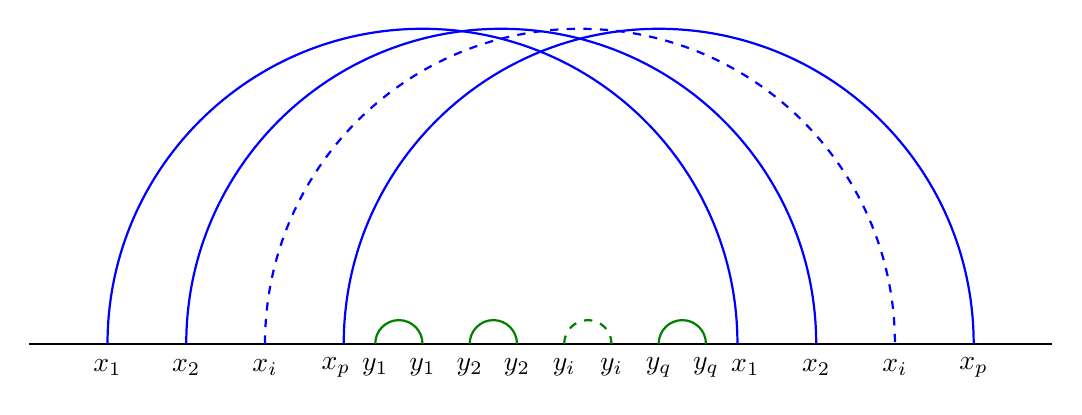
\begin{tikzpicture}
			\draw[thick] (0,0) -- (13,0);
			\draw[color=Blue, thick] (1,0) arc (180:0:4);
			\draw[color=Blue, thick] (2,0) arc (180:0:4);
			\draw[color=Blue, thick, dashed] (3,0) arc (180:0:4);
			\draw[color=Blue, thick] (4,0) arc (180:0:4);
			\draw[color=Green, thick] (4.4,0) arc (180:0:.3);
			\draw[color=Green, thick] (5.6,0) arc (180:0:.3);
			\draw[color=Green, thick, dashed] (6.8,0) arc (180:0:.3);
			\draw[color=Green, thick] (8,0) arc (180:0:.3);
			\node at (1, -.3) {$x_1$};
			\node at (2, -.3) {$x_2$};
			\node at (3, -.3) {$x_i$};
			\node at (3.9, -.3) {$x_p$};
			\node at (4.4, -.3) {$y_1$};
			\node at (5, -.3) {$y_1$};
			\node at (5.6, -.3) {$y_2$};
			\node at (6.2, -.3) {$y_2$};
			\node at (6.8, -.3) {$y_i$};
			\node at (7.4, -.3) {$y_i$};
			\node at (8, -.3) {$y_q$};
			\node at (8.6, -.3) {$y_q$};
			\node at (9.1, -.3) {$x_1$};
			\node at (10, -.3) {$x_2$};
			\node at (11, -.3) {$x_i$};
			\node at (12, -.3) {$x_p$};
		\end{tikzpicture}
		\caption{Definice $(p-q)$-konfigurace.}
		\label{konf}
	\end{figure}
\end{defn}

\begin{notation}
	$\text{CIR}(k,p,q) = \{G \in \text{CIR}, \omega(G) \leq k, G \text{ má reprezentaci bez } (p,q)\text{-konfigurace}\}$.
\end{notation}

\begin{observ}
	Pro $p > k$ a libovolné $q \in \N_0$: $\text{CIR}(k,p,q) = \text{CIR}(k)$.
\end{observ}

\begin{claim}
	$\forall k \in \N \ \forall p, q \in \N_0 \ \exists g(k,p,q) \in \N$ t.ž. $\forall G \in \text{CIR}(k,p,q) : \chi(G) \leq g(k,p,q)$.
\end{claim}

\begin{observ}
	Důkazem tohoto tvrzení platí věta.
\end{observ}

\begin{proof}
	Dané tvrzení dokážeme pomocí dvojité indukce: Indukcí podle $p \in \N_0$:
	
	\begin{lemma}
		$\forall G \in \text{CIR}(k,0,q) : \chi (G) \leq k (q-1)$ pro $q \geq 2$.
	\end{lemma}
	
	\begin{proof}[Proof of lemma]
		Indukcí podle $q \in \N_0$. Pokud $q = 2$ tak můžeme pozorovat, že všechny obloučky protínají společnou souvislou přímku. Tím pádem $\forall k : \text{CIR}(k,0,2) \subseteq \text{PER}$ které jsou perfektní.
		
		Nyní nechť $q > 2$. Nechť $G \in \text{CIR}(k, 0, q)$, vrcholy $G$ rozdělíme na 2 části $V_1, V_2$ tak, že
		
		\begin{itemize}
			\item $V_1$ bude indukovat graf z $\text{CIR}(k,0,2)$ a
			\item $V_2$ bude indukovat graf z $\text{CIR}(k,0,q-1)$.
		\end{itemize}
		
		Označme $\pi$ jakožto nejpravější levý konec obloučku. Potom $V_1$ jsou vrcholy, které mají levý konec vlevo od $\pi$. A $V_2$ jsou vrcholy, které mají levý konec napravo od $\pi$. Pak už použijeme indukci.
	\end{proof}
	
	\begin{lemma}
		Nechť $p \geq 1, q \geq 1$. Potom $\forall G \in \text{CIR}(k,p,q):$ vrcholy $G$ lze rozdělit na 2 části $V_A, V_B$ tak, že každá komponenta $G[V_A]$ i $G[V_B]$ patří do $\text{CIR}(k, p-1, 2q+1)$.
	\end{lemma}
	
	\begin{cor}
		Lze vzít $g(k,p,q) = g (k, p-1, 2q+1)$ tedy tvrzení pak platí.
	\end{cor}
	
	\begin{proof}[Proof of lemma]
		Mějme $G \in \text{CIR}(k,p,q)$. BÚNO: $G$ je souvislý a máme danou reprezentaci. Nechť $x_0$ je vrchol $G$ jehož oblouček má nejlevější levý konec. Definujeme $V_i := \{x \in V(G) : \text{ nejkratší cesta v } G \text{ od } x_0 \text{ do } x$ má délku $i\}$.
		
		\begin{observ}
			Pokud vede hrana z $V_i$ do $V_j$ tak $|i - j| \leq 1$.
		\end{observ}
		
		\begin{observ}
			Z každého vrcholu $V_{i+1}$ vede aspoň 1 hrana do $V_i$.
		\end{observ}
		
		Nyní tvrdíme, že žádná komponenta $G[V_i]$ neobsahuje $(p-1, 2q + 1)$-konfiguraci.
		
		Nechť $C$ je komponenta $G[V_i]$ pro spor obsahující $(p-1, 2q + 1)$-konfiguraci. Označme $y_{q+1}$ nějaký oblouček $w$ musí protnout $y_{q+1}$, tedy $w \in V_{i-1}$. Aspoň jeden konec je mimo $C$. $V_{i-1} = V_0$ tedy hotovo. Kdyby měl oba konce v $C$, tak nelze protnout oblouček z $V_{i-2}$.
		
		Nyní nechť $x_1, \dots, x_{p-1}, y_{1}, \dots, y_{2q+1}$ je $(p-1, 2q + 1)$-konfigurace. Nechť $I$ je interval mezi nejlevějším a nejpravějším koncem obloučku v $C$.
		
		\begin{observ}
			Každý soused $w \in V_{i-1}$ vrcholu $y_{q+1}$ musí mít jeden konec mimo $I$.
		\end{observ}
		
		Potom $w, x_1, \dots, x_{p-1}, y_{1}, \dots, y_q$ nebo $w, x_1, \dots, x_{p-1}, y_{q+2}, \dots, y_{2q+1}$ je $(p,q)$-konfigurace v $G$, což je spor.
		
		Závěrem $V_{A} := \cup_{i \text{ sudé}} V_{i}$ a $V_{B} := \cup_{i \text{ liché}} V_{i}$.
	\end{proof}
\end{proof}

\section{$\chi$-unboundedness of SEG graphs}

\begin{defn}
	SEG is the class of graphs of intersection graphs of segments in the plane.
\end{defn}

Now the question might be if SEG graphs are $\chi$-bounded or not. This was firstly stated by Erdös. The answer came later by the following theorem.

\begin{thm}[Pawlik, Kozik, Krawczyk, Lagos, Micek, Trotter, Wolezak, 2012]
	$\forall k \in \N$ there exists triangle-free graph $G_k \in \text{SEG}$ with $\chi(G_k) \geq k$.
	\label{PKKLMTW thm}
\end{thm}

\begin{defn}
	\textbf{L-curve} is a union of a horizontal and vertical segment sharing a common bottom-left endpoint. \textbf{L-graph} is an intersection graph of L-curves.
\end{defn}

\begin{thm}
	Any L-graph is also SEG-graph.
\end{thm}

\begin{proof}
	Suppose $\mathcal{L} = \{l_1, l_2, \dots, l_n\}$ is a set of L-curves, we will show by induction on $\abs{\mathcal{L}} = n$ that there is a set $\mathcal{S} = \{s_1, s_2, \dots, s_n\}$ of segments s.t. $l_i \cap l_j \neq \emptyset \Leftrightarrow s_i \cap s_j \neq \emptyset$, and moreover:
	
	\begin{enumerate}
		\item all $s_1, \dots, s_n$ lie in the half plane below the $x$-axis;
		\item $s_i$ touches the $x$-axis \ifft $l_i$ can be extended upwards to infinity without crossing any other $l_j \in \mathcal{L}$;
		\item left-to-right order of $s_i$'s touching the $x$-axis is the same as for $l_i$'s.
	\end{enumerate}
	
	Now for $n = 1$ it is simple, see Fig. \ref{start-l-curves}, and for $n > 1$ \wlogt $l_n$ has topmost horizontal part. By induction we represent $\mathcal{L}' = \{l_1, \dots, l_{n-1}\}$ by $\mathcal{S}' = \{s_1, \dots, s_{n-1}\}$ then
	
	\begin{enumerate}
		\item shorten the $s_i$ if $l_i$ no longer can extend upwards and
		\item insert $s_n$ touching $x$-axis, nearly horizontal. See Fig. \ref{induction-l-curves}.
	\end{enumerate}
	
	\begin{figure}[!ht]\centering
		\begin{subfigure}{.45\textwidth}\centering
			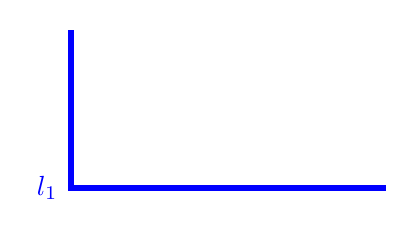
\begin{tikzpicture}[l/.style = {line width = 2pt}, b/.style = {Blue}]
				\draw[l, b] (0,2) to[out=270, in=90] (0,0) to[out=0, in=180] (4,0);
				\node[b] at (-.3,0) {$l_1$};
			\end{tikzpicture}
			\caption{L-curves.}
		\end{subfigure}
		\begin{subfigure}{.45\textwidth}\centering
			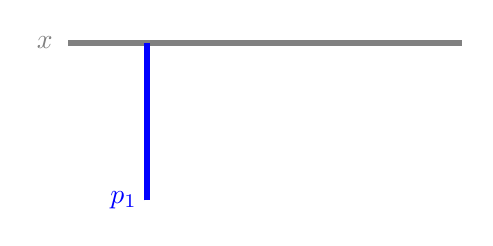
\begin{tikzpicture}[l/.style = {line width = 2pt}, b/.style = {Blue}]
				\draw[l, gray] (0,0) -- (5,0);
				\node[gray] at (-.3,0) {$x$};
				\draw[l, b] (1, -2) -- (1,0);
				\node[b] at (.7, -2) {$p_1$};
			\end{tikzpicture}
			\caption{Segments.}
		\end{subfigure}
		\caption{Simple of start for an induction.}
		\label{start-l-curves}
	\end{figure}
	
	\begin{figure}[!ht]\centering
		\begin{subfigure}{.45\textwidth}\centering
			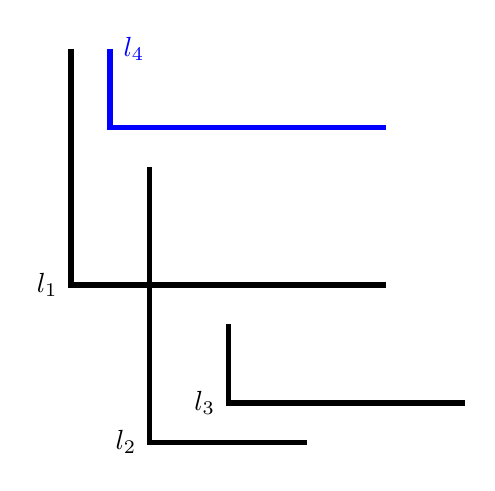
\begin{tikzpicture}[l/.style = {line width = 2pt}]
				\draw[l] (0,3) to[out=270, in=90] (0,0) to[out=0, in=180] (4,0);
				\node at (-.3,0) {$l_1$};
				\draw[l] (1,1.5) to[out=270, in=90] (1,-2) to[out=0, in=180] (3,-2);
				\node at (.7,-2) {$l_2$};
				\draw[l] (2,-.5) to[out=270, in=90] (2,-1.5) to[out=0, in=180] (5,-1.5);
				\node at (1.7,-1.5) {$l_3$};
				\draw[l, Blue] (.5,3) to[out=270, in=90] (.5,2) to[out=0, in=180] (4,2);
				\node[Blue] at (.8,3) {$l_4$};
			\end{tikzpicture}
			\caption{L-curves.}
		\end{subfigure}
		\begin{subfigure}{.45\textwidth}\centering
			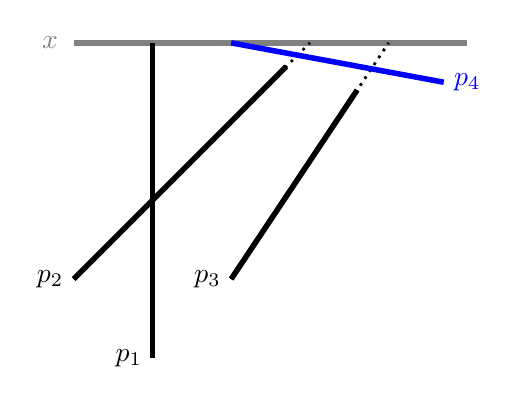
\begin{tikzpicture}[l/.style = {line width = 2pt}]
				\draw[l, gray] (0,0) -- (5,0);
				\node[gray] at (-.3,0) {$x$};
				\draw[l] (1, -4) -- (1,0);
				\node at (.7, -4) {$p_1$};
				\draw[l] (0, -3) -- (2.7,-.3);
				\draw[dotted, line width = 1pt] (0, -3) -- (3,0);
				\node at (-.3, -3) {$p_2$};
				\draw[l] (2, -3) -- (3.6,-.6);
				\draw[dotted, line width = 1pt] (2, -3) -- (4,0);
				\node at (1.7, -3) {$p_3$};
				\draw[l, Blue] (4.7, -.5) -- (2,0);
				\node[Blue] at (5, -.5) {$p_4$};
			\end{tikzpicture}
			\caption{Segments.}
		\end{subfigure}
		\caption{Simple example for conversion.}
		\label{induction-l-curves}
	\end{figure}
\end{proof}

\begin{proof}[Proof of theorem \ref{PKKLMTW thm}]
	In fact we show that $\forall k \in \N$ there exists triangle-free L-graph $G_k$ with $\chi(G_k) \geq k$.
	
	\begin{defn}
		A \textit{configuration} is
		
		\begin{enumerate}
			\item a collection of L-curves inside the unit square $[0,1] \times [0,1]$, whose intersection graph is triangle-free;
			\item a set $\{P_1, \dots, P_m\}$ of \textit{"probes"} which are pairwise disjoint rectangles inside $[0,1] \times [0,1]$ touching its bottom boundary;
			\item any L-shape from the collection intersecting a probe $P_i$ must cross it from left to right; \label{conf-3}
			\item the L-shape crossing a given probe are pairwise disjoint. \label{conf-4}
		\end{enumerate}
		
		\begin{figure}[!ht]\centering
			\begin{subfigure}{.45\textwidth}\centering
				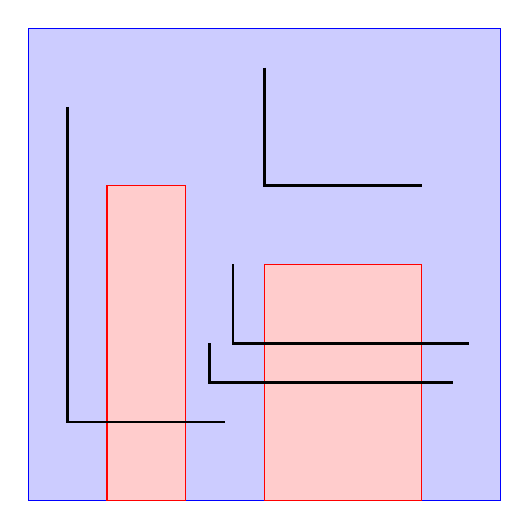
\begin{tikzpicture}[l/.style = {line width = 1pt}]
					\draw[Blue, fill=Blue!20] (0,0) rectangle (6,6);
					\draw[Red, fill=Red!20] (1,0) rectangle (2,4);
					\draw[Red, fill=Red!20] (3,0) rectangle (5,3);
					\draw[l] (.5,5) to[out=270, in=90] (.5,1) to[out=0, in=180] (2.5,1);
					\draw[l] (2.3,2) to[out=270, in=90] (2.3,1.5) to[out=0, in=180] (5.4,1.5);
					\draw[l] (2.6,3) to[out=270, in=90] (2.6,2) to[out=0, in=180] (5.6,2);
					\draw[l] (3,5.5) to[out=270, in=90] (3,4) to[out=0, in=180] (5,4);
				\end{tikzpicture}
				\caption{Example of configuration where we have \textcolor{Red}{two probes} in a \textcolor{Blue}{[0,1] box} with four L-curves.}
			\end{subfigure}
			\begin{subfigure}{.45\textwidth}\centering
				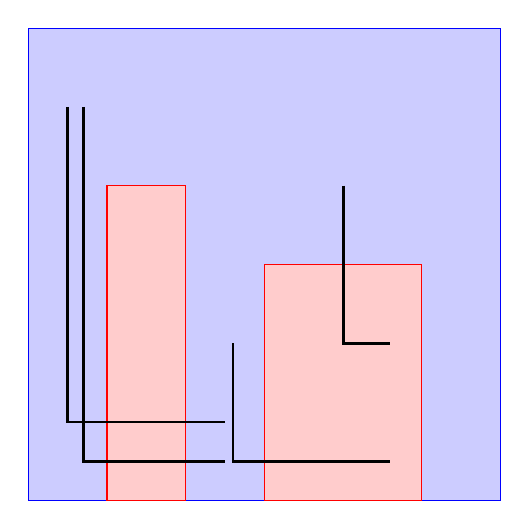
\begin{tikzpicture}[l/.style = {line width = 1pt}]
					\draw[Blue, fill=Blue!20] (0,0) rectangle (6,6);
					\draw[Red, fill=Red!20] (1,0) rectangle (2,4);
					\draw[Red, fill=Red!20] (3,0) rectangle (5,3);
					\draw[l] (2.6,2) to[out=270, in=90] (2.6,.5) to[out=0, in=180] (4.6,.5);
					\draw[l] (4,4) to[out=270, in=90] (4,2) to[out=0, in=180] (4.6,2);
					\draw[l] (.5,5) to[out=270, in=90] (.5,1) to[out=0, in=180] (2.5,1);
					\draw[l] (.7,5) to[out=270, in=90] (.7,.5) to[out=0, in=180] (2.5,.5);
				\end{tikzpicture}
				\caption{Counterexample of violating the definitions \ref{conf-3} and \ref{conf-4}.}
			\end{subfigure}
			\caption{Example and counterexamples of the definition.}
		\end{figure}
	\end{defn}
	
	We will construct two sequences of $A_1, A_2, A_3, \dots$ and $B_1, B_2, B_3, \dots$ of configurations s.t.:
	
	\begin{enumerate}
		\item $\forall k \in \N$ in any proper coloring of the L-curves in $A_k$, the L-curves seen inside the probes use at least $k$ different colors.
		\item $\forall k \in \N$ in any proper coloring of the L-curves in $B_k$ there exist a probe of $B_k$ which is crossed by L-curves of at least $k$ different colors.
	\end{enumerate}
	
	By induction for $k = 1$ it is straightforward, see Fig. \ref{start-configuration}. Now we show two parts.
	
	\begin{figure}[!ht]\centering
		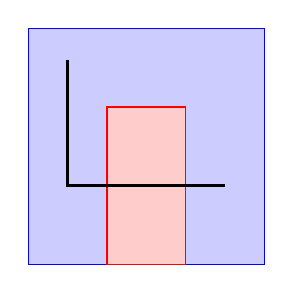
\begin{tikzpicture}[l/.style = {line width = 1pt}]
			\draw[Blue, fill=Blue!20] (0,0) rectangle (3,3);
			\draw[Red, fill=Red!20] (1,0) rectangle (2,2);
			\draw[l] (.5,2.6) to[out=270, in=90] (.5,1) to[out=0, in=180] (2.5,1);
		\end{tikzpicture}
		\caption{Start of the induction with \textcolor{Red}{one probe} and one L-curve.}
		\label{start-configuration}
	\end{figure}
	
	\begin{enumerate}
		\item From $B_k$ to $A_k+1$. See Fig. \ref{ak+1}.
		\begin{enumerate}
			\item Insert one new L-shape inside every probe of $B_k$ and
			\item replace each probe by 2 new probes.
		\end{enumerate}
		\item From $B_k$ and $A_{k+1}$ to $B_{k+1}$. See Fig. \ref{bk+1}.
		\begin{enumerate}
			\item Insert a small copy of $A_{k+1}$ near the top of every probe of $B_k$ and
			\item extend the probes of these small copies all the way down to obtain probes of $B_{k+1}$.
		\end{enumerate}
	\end{enumerate}
	
	\begin{figure}[!ht]\centering
		\begin{subfigure}{.45\textwidth}\centering
			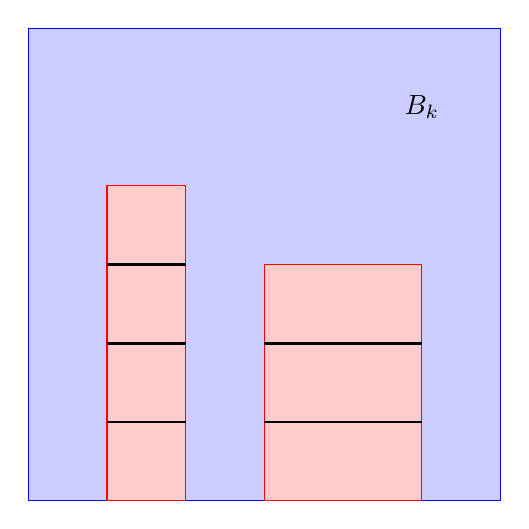
\begin{tikzpicture}[l/.style = {line width = 1pt}]
				\draw[Blue, fill=Blue!20] (0,0) rectangle (6,6);
				\draw[Red, fill=Red!20] (1,0) rectangle (2,4);
				\draw[Red, fill=Red!20] (3,0) rectangle (5,3);
				\draw[l] (1,1) to (2,1);
				\draw[l] (1,2) to (2,2);
				\draw[l] (1,3) to (2,3);
				\draw[l] (3,1) to (5,1);
				\draw[l] (3,2) to (5,2);
				\node at (5,5) {$B_k$};
			\end{tikzpicture}
			\caption{Simplification with \textcolor{Red}{two probes}.}
		\end{subfigure}
		\begin{subfigure}{.45\textwidth}\centering
			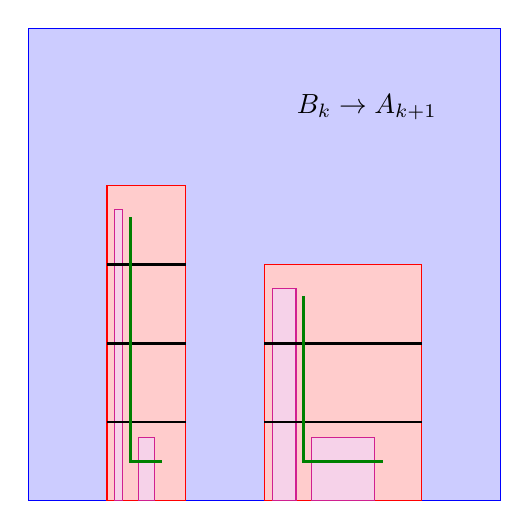
\begin{tikzpicture}[l/.style = {line width = 1pt}]
				\draw[Blue, fill=Blue!20] (0,0) rectangle (6,6);
				\draw[Red, fill=Red!20] (1,0) rectangle (2,4);
				\draw[Red, fill=Red!20] (3,0) rectangle (5,3);
				\draw[VioletRed, fill=VioletRed!20] (1.1,0) rectangle (1.2,3.7);
				\draw[VioletRed, fill=VioletRed!20] (1.4,0) rectangle (1.6,.8);
				\draw[l] (1,1) to (2,1);
				\draw[l] (1,2) to (2,2);
				\draw[l] (1,3) to (2,3);
				\draw[l, Green] (1.3,3.6) to[out=270, in=90] (1.3,.5) to[out=0, in=180] (1.7,.5);
				\draw[VioletRed, fill=VioletRed!20] (3.1,0) rectangle (3.4,2.7);
				\draw[VioletRed, fill=VioletRed!20] (3.6,0) rectangle (4.4,.8);
				\draw[l] (3,1) to (5,1);
				\draw[l] (3,2) to (5,2);
				\draw[l, Green] (3.5,2.6) to[out=270, in=90] (3.5,.5) to[out=0, in=180] (4.5,.5);
				\node at (4.3,5) {$B_k \to A_{k+1}$};
			\end{tikzpicture}
			\caption{\textcolor{Green}{Two new L-curves} and \textcolor{VioletRed}{four new probes}.}
		\end{subfigure}
		\caption{Conversion from $B_k$ to $A_{k+1}$.}
		\label{ak+1}
	\end{figure}
	
	\begin{figure}[!ht]\centering
		\begin{subfigure}{.45\textwidth}\centering
			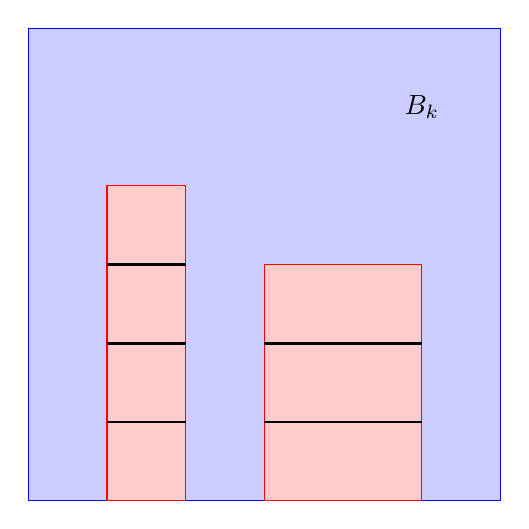
\begin{tikzpicture}[l/.style = {line width = 1pt}]
				\draw[Blue, fill=Blue!20] (0,0) rectangle (6,6);
				\draw[Red, fill=Red!20] (1,0) rectangle (2,4);
				\draw[Red, fill=Red!20] (3,0) rectangle (5,3);
				\draw[l] (1,1) to (2,1);
				\draw[l] (1,2) to (2,2);
				\draw[l] (1,3) to (2,3);
				\draw[l] (3,1) to (5,1);
				\draw[l] (3,2) to (5,2);
				\node at (5,5) {$B_k$};
			\end{tikzpicture}
			\caption{Simplification with \textcolor{Red}{two probes}.}
		\end{subfigure}
		\begin{subfigure}{.45\textwidth}\centering
			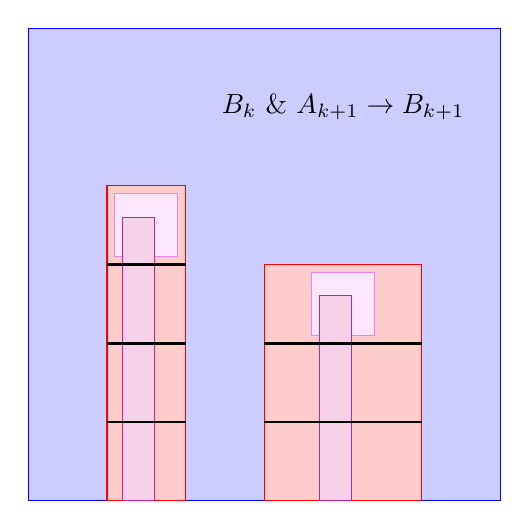
\begin{tikzpicture}[l/.style = {line width = 1pt}]
				\draw[Blue, fill=Blue!20] (0,0) rectangle (6,6);
				\draw[Red, fill=Red!20] (1,0) rectangle (2,4);
				\draw[Red, fill=Red!20] (3,0) rectangle (5,3);
				\draw[Violet, fill=Violet!20] (1.1, 3.1) rectangle (1.9, 3.9);
				\draw[VioletRed, fill=VioletRed!20] (1.2, 0) rectangle (1.6, 3.6);
				\draw[Violet, fill=Violet!20] (3.6, 2.1) rectangle (4.4, 2.9);
				\draw[VioletRed, fill=VioletRed!20] (3.7, 0) rectangle (4.1, 2.6);
				\draw[l] (1,1) to (2,1);
				\draw[l] (1,2) to (2,2);
				\draw[l] (1,3) to (2,3);
				\draw[l] (3,1) to (5,1);
				\draw[l] (3,2) to (5,2);
				\node at (4,5) {$B_k \ \& \ A_{k+1} \to B_{k+1}$};
			\end{tikzpicture}
			\caption{\textcolor{Violet}{Copies of $A_{k+1}$} and \textcolor{VioletRed}{prolonged probes}.}
		\end{subfigure}
		\caption{Conversion from $A_{k+1}$ and $B_{k}$ to $B_{k+1}$.}
		\label{bk+1}
	\end{figure}
\end{proof}

Now we may ask ourselves if this prove can be extended to some other type of intersection graphs. Well indeed it can be done. Note that \textit{arc-connected} set means that all pairs from the set can be connected via an arc.

\begin{fact}
	For any compact arc-connected set $X \subseteq \R^2$ other then an axis parallel rectangle there is a triangle-free graph $G_k$, $\chi(G_k) \geq k$, which is the intersection graph of horizontally and vertically scaled copies of $X$.
\end{fact}

\begin{defn}
	A graph $G$ is $d$-degenerate if every non-empty subgraph of $G$ contains a vertex of degree at most $d$.
\end{defn}

\begin{observ}
	$G$ is $d$-degenerate then $\chi(G) \leq d+1$.
\end{observ}

\begin{proof}
	This observation can be seen by induction. Lets take $u$ which has $\deg(u) \leq d$ now take $G - u$ which is also $d$-degenerate and therefore by induction hypothesis colorable by $d+1$ colors. Lets take such coloring and now give $u$ a possible color. Because it only has $d$ neighbors we will have at least 1 possibility.
\end{proof}

\section{Axis-parallel rectangles intersection graphs}

\begin{thm}[Asblund, Grunbaum]
	If $G$ is an intersection graph of axis parallel rectangles in the plane then $\chi(G) \leq O(\omega^2 (G))$.
\end{thm}

\begin{proof}
	Suppose we have $G = (V,E)$ as above: each vertex $u \in V$ is represented by a rectangle $R_u$. Let $E = E_1 \dot{\cup} E_2$ as follows
	
	\begin{enumerate}
		\item $\{u,v\} \in E_1$ if a vertex of $R_u$ is inside $R_v$ or vice versa (Fig. \ref{inter-box})
		\item $E_2 = E \setminus E_1$ if it is cross-like (Fig. \ref{cross-box}).
	\end{enumerate}
	
	\begin{figure}[!ht]\centering
		\begin{subfigure}{.45\textwidth}\centering
			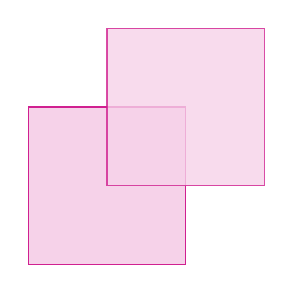
\begin{tikzpicture}
				\draw[VioletRed, fill=VioletRed!20] (0, 0) rectangle (2, 2);
				\draw[VioletRed, fill=VioletRed!20, opacity=0.8] (1, 1) rectangle (3, 3);
			\end{tikzpicture}
			\caption{One vertex is inside the other rectangle.}
			\label{inter-box}
		\end{subfigure}
		\begin{subfigure}{.45\textwidth}\centering
			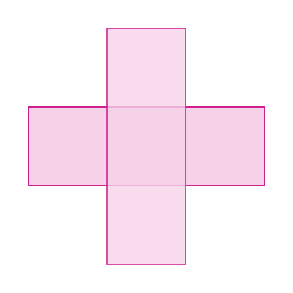
\begin{tikzpicture}
				\draw[VioletRed, fill=VioletRed!20] (0, 1) rectangle (3, 2);
				\draw[VioletRed, fill=VioletRed!20, opacity=0.8] (1, 0) rectangle (2, 3);
			\end{tikzpicture}
			\caption{Cross-like intersection.}
			\label{cross-box}
		\end{subfigure}
		\caption{Two possibilities.}
	\end{figure}
	
	Lets denote $G_1 = (V, E_1)$, $G_2 = (V, E_2)$ and $k = \omega(G)$. We will show $\chi(G_1) = O(k)$ and $\chi(G_2) = O(k)$.
	
	\begin{itemize}
		\item For $G_1$ we claim that $|E_1| \leq 4 k \cdot |V|$ (and any subgraph of $G_1$ induced by $W \subseteq V$ has at most $4 k \cdot |W|$ edges). This is because each vertex of a rectangle is inside at most $k-1$ other rectangles, due to the maximal clique. So this means one for each vertex of a rectangle is in total $4 (k-1)$. Now we direct an edge $uv$ if vertex of $R_u$ is inside $R_v$. Thus the outdegree of any vertex is $\leq 4 (k-1)$ so $|E_1| \leq 4 (k-1) \cdot |V|$. Hence $G_1$ (and any of its induced subgraphs) has average degree $\frac{2 |E_1|}{|V|} = 8 (k-1)$. So the min degree is $\leq 8 (k-1)$ therefore it is $8(k-1)$-degenerate and hence $\chi(G_1) \leq 8 (k-1) + 1$.
		\item For $G_2$ we claim that $\chi(G_2) = \omega(G_2) = O(k)$ because $G_2$ is a comparability graph (for example sort the boxes from tallest to shortest).
		\item For $G$ we have $\chi(G) \leq \chi(G_1) \cdot \chi(G_2) = O(k^2)$. For this lets have $E_1 \dot{\cup} E_2$ and see Fig. \ref{two-colors}. That is we have coloring $1,2, \dots, p$ colors for $E_1$ and $1,2, \dots, q$ colors for $E_2$ and we create a coloring by tuples $(x,y)$ where $x \in [p]$ and $y \in [q]$.
	\end{itemize}
	
	\begin{figure}[!ht]\centering
		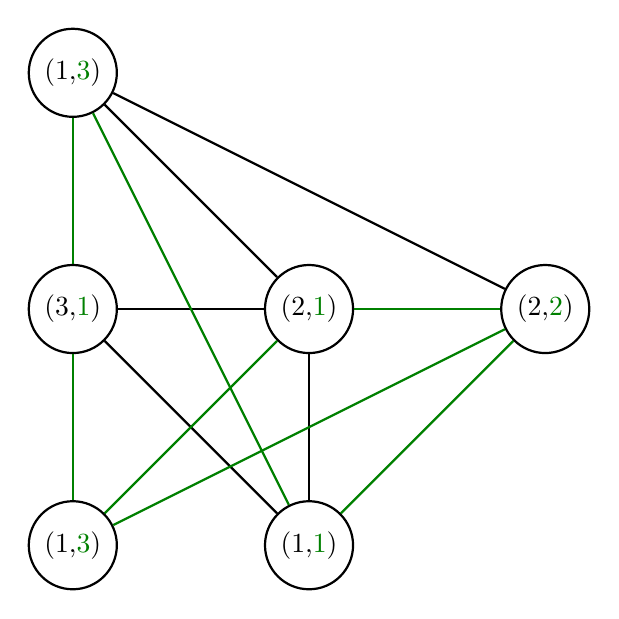
\begin{tikzpicture}[node distance = 30mm, main/.style = {draw, circle, thick}]
			\node[main] (0) {(1,\textcolor{Green}{1})};
			\node[main, above of = 0] (1) {(2,\textcolor{Green}{1})};
			\node[main, left of = 1] (2) {(3,\textcolor{Green}{1})};
			\node[main, right of = 1] (3) {(2,\textcolor{Green}{2})};
			\node[main, left of = 0] (4) {(1,\textcolor{Green}{3})};
			\node[main, above of = 2] (5) {(1,\textcolor{Green}{3})};
			\draw[thick] (0) -- (1);
			\draw[thick] (0) -- (2);
			\draw[thick] (1) -- (2);
			\draw[thick] (1) -- (5);
			\draw[thick, Green] (0) -- (3);
			\draw[thick, Green] (0) -- (5);
			\draw[thick, Green] (1) -- (4);
			\draw[thick, Green] (1) -- (3);
			\draw[thick, Green] (2) -- (4);
			\draw[thick, Green] (2) -- (5);
			\draw[thick, Green] (3) -- (4);
			\draw[thick] (3) -- (5);
		\end{tikzpicture}
		\caption{Disjoint union of edges for coloring.}
		\label{two-colors}
	\end{figure}
\end{proof}

\section{1-String with big girth}

Now we will continue further and see that L-graphs $\subseteq$ (proper, i.e. not overlapping segments) SEG $\subseteq$ 1-String $\subseteq$ String. For this we need to see the definitions first.

\begin{defn}
	$G \in$ 1-String if $G$ has a String representation in which every two strings intersect at most once.
\end{defn}

\begin{defn}
	The \textbf{girth} of a graph $G$ is the length of the shortest cycle in $G$, if $G$ has no cycle then girth is $+ \infty$. We will denote girth of $G$ as $\gamma(G)$.
\end{defn}

With the newly established terminology we have previously shown that L-graphs of girth $\geq 4$ have unbounded $\chi$, but what about girth $\geq 5$ (or $6, \dots$). Also we will give a remark which is that for arbitrary large girth and chromatic number can be created. This can be shown by probabilistic techniques.

\begin{thm}[Kostochka \& Nešetřil]
	Let $G$ be a 1-String graph, then
	$$
	\begin{array}{r c l r}
		\text{if } \gamma(G) \geq 5 & \Rightarrow & \chi(G) \leq 6 & (\text{degeneracy } \leq 5), \\
		\text{if } \gamma(G) \geq 6 & \Rightarrow & \chi(G) \leq 4 & (\text{degeneracy } \leq 3), \\
		\text{if } \gamma(G) \geq 8 & \Rightarrow & \chi(G) \leq 3 & (\text{degeneracy } \leq 2). \\
	\end{array}
	$$
\end{thm}

\begin{proof}
	Let $G = (V,E)$ be a connected 1-String graph, with a given 1-String representation. $n = |V|, m = |E|$. We will show the minimal degree of this graph where the degeneracy will follow, since its subgraphs can only have larger girth. Let $H = (V_H, E_H)$ be a plane graph whose drawing is obtained by placing a vertex on every crossing of strings of $G$, pieces of string between adjacent crossings are the edges of $H$. Recall Euler's formula $v - e + f = 2 \geq 0$.
	
	$$
	\begin{aligned}
		&v = |V_H| = \frac{1}{2} \sum_{v \in V} \deg(v) = m \\
		&e = |E_H| = \sum_{w \in V}(\deg(w) - 1) = \left(\sum_{w \in V} \deg (w)\right) - n = 2m - n \\
		&f = \text{\# of faces of } H
	\end{aligned}
	$$
	
	\begin{observ}
		If $H$ has a face bounded by a cycle of length $l$, then $G$ has a closed walk of length $l$ in which each edge appears at most once. Hence $\gamma(G) \leq l$.
	\end{observ}
	
	And consequently every face of $H$ is incident to at least $\gamma(G)$ edges of $H$. Hence $f \cdot \gamma(G) \leq 2 e$.
	
	$$
	f \leq \frac{2e}{\gamma(G)} = \frac{4m - 2n}{\gamma(G)}
	$$
	
	So we can use the following computation.
	
	$$
	0 < v - e + f \leq m - 2m + n + \frac{4m - 2n}{\gamma(G)} = n \left(1 - \frac{2}{\gamma(G)} \right) - m \left(1 - \frac{4}{\gamma(G)} \right)
	$$
	
	\noindent This enforces the following.
	
	$$
	m \left(1 - \frac{4}{\gamma(G)}\right) < n \left(1 - \frac{2}{\gamma(G)} \right)
	$$
	
	\noindent Thus the min. degree $\leq$ average degree which is
	
	$$
	= \frac{2m}{n} \leq \frac{2 \left(1 - \frac{2}{\gamma(G)} \right)}{\left(1 - \frac{4}{\gamma(G)}\right)} = \frac{2 (\gamma(G) -2)}{\gamma(G) - 4}
	$$
	
	\noindent Lastly we compute the exact values. If $\gamma(G) \geq 5$ then min degree $< 6$ so $\leq 5$ hence $\chi(G) \leq 6$. If $\gamma(G) \geq 6$ then min degree $< 4$ so $\leq 3$ hence $\chi(G) \leq 4$. If $\gamma(G) \geq 8$ then min degree $< 3$ so $\leq 2$ hence $\chi(G) \leq 3$.
\end{proof}

Now we will further generalize to String graphs, which will use completely new topic which is called Game of robber and cops. Note that there exists more versions of this game.

\section{Game of robber and cops}

We have a given graph $G$. Then 1 robber (\textcolor{Red}{\faCircle}) and $c$ cops (\textcolor{Green}{\faSquare}). This game is for 2 players. Both players take turns. First one plays with cops and the second with robber.

\begin{mybox}{Rules}
	\begin{itemize}[]
		\item \textbf{Start of the game:} First player places cops on vertices of graph $G$. Then second player places the robber on some vertex.
		\item \textbf{Single turn:} First player can with each cop either move to adjacent vertex or stay in the same one. Then the robber can move to adjacent or stay in the same vertex.
		\item \textbf{Goal:} If both cop and robber end up in the same vertex cops have won. Alternatively robber wants to stay as long as possible.
	\end{itemize}
\end{mybox}

\begin{example}
	We have an easy example of the given graph and robber and cops. See Fig. \ref{cops-robber}
	
	\begin{figure}[!ht]\centering
		\begin{tikzpicture}[node distance = 15mm, main/.style = {draw, circle}, thick]
			\node[main] (0) {\textcolor{Green}{\faSquare}};
			\node[main, below of = 0] (1) {\textcolor{Green}{\faSquare}};
			\node[main, left of =1] (2) {};
			\node[main, right of =1] (3) {};
			\node[main, below of =1] (4) {};
			\node[main, left of=4] (5) {\textcolor{Green}{\faSquare} \textcolor{Green}{\faSquare}};
			\node[main, right of=4] (6) {\textcolor{Red}{\faCircle}};
			\node[main, below of =6] (7) {};
			\draw (0) -- (1);
			\draw (1) -- (2);
			\draw (0) -- (2);
			\draw (1) -- (3);
			\draw (0) -- (3);
			\draw (1) -- (4);
			\draw (2) -- (4);
			\draw (3) -- (4);
			\draw (5) -- (4);
			\draw (6) -- (4);
			\draw (7) -- (4);
			\draw (7) -- (6);
			\draw (2) -- (5);
		\end{tikzpicture}
		\caption{Example for cops and robber game.}
		\label{cops-robber}
	\end{figure}
\end{example}



\begin{defn}
	The \textbf{cop-number} $\cn(G) :=$ smallest number of cops for which the cops have a winning strategy on $G$. And for class $\mathcal{C}$ of graphs we define $\cn(\mathcal{C}) := \sup \{\cn (G), G \in \mathcal{C}, G \text{ connected}\}$.
\end{defn}

\begin{example}[Cycles]
	For cycles $C_n$ with $n \geq 4$ we can easily see that $\cn(G) = 2$ because we may put two cops in one vertex and then enclose the circle by two pats. Alternatively one is not enough since the robber may only wait and if cop is in the neighboring vertex the robber moves away.
\end{example}

\begin{example}[Int]
	In Int which is class of interval graphs we may find out that $\cn(\text{Int}) = 1$. Firstly we sort the intervals by its left endpoints, then place cop in the leftmost interval. The strategy is either catch a robber or move right to the next interval. If robber could move away the robber must stay way apart to the right or left. But note that if he would be in the left we didn't follow our strategy.
	
	Alternatively we can say the Int has a clique-path decomposition and in each step we are either in the same clique so we can catch the robber or we may move to the next clique.
\end{example}

\begin{prop}
	Let $G$ be a graph with $\gamma(G) \geq 5$. If every vertex of $G$ has degree $\geq d$, then $\cn(G) \geq d$.
	\label{girth-cop}
\end{prop}

\begin{proof}
	If $v$ is the robbers current vertex and $v_1, v_2, \dots, v_k$ are the neighbours of $v$, then each cop can be in the closed neighbourhood of at most one of $v_1, v_2, \dots, v_k$. If $k > \#$ of cops, robber may move to a "safe" neighbour $v_i$ if needed.
\end{proof}

\begin{cons}
	If $\mathcal{C}$ is a class of graphs closed under induced subgraphs with $\cn(\mathcal{C}) = c < + \infty$, then every graph $G \in \mathcal{C}$ of girth $\geq 5$ is $c$-degenrate and hence $\chi(G) \leq c+1$.
\end{cons}

\begin{thm}[Das and Gahlawat, 2022]
	$\cn(\text{String}) \leq 13$.
\end{thm}

We won't show this theorem. Also the lower bound is known to be 3. And String graphs of girth $\geq 5$ have $\chi \leq 14$ which follows from the theorem and proposition \ref{girth-cop}.

\begin{thm}
	$\cn(\text{Outer planar}) \in \{3,4\}$.
\end{thm}

\begin{proof}[Proof of the lower bound]
	We may construct a so called "$3 \times 5$ grid" see Fig. \ref{grid} for the graph itself and a representation. Then if 2 cops are adjacent to the robber then there is always one vertex for "lazy strategy" robber.
	
	\begin{figure}[!ht]\centering
		\begin{subfigure}{.45\textwidth}\centering
			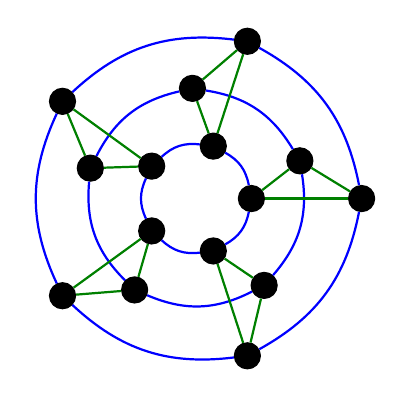
\begin{tikzpicture}[scale=.7]
				\foreach \i in {1,...,5} {
					\node[draw, circle, fill] (O-\i) at ({360/5 * (\i-1)}:3) {};
			    	}
				\foreach \i in {1,...,4} {
					\pgfmathtruncatemacro{\j}{\i+1}
					\draw[thick, Blue, bend right = 25] (O-\i) edge (O-\j);
				}
				\draw[thick, Blue, bend right = 25] (O-5) edge (O-1);
			       	\foreach \i in {1,...,5} {
			    		\node[draw,circle, fill] (M-\i) at ({360/5 * (\i-1) + 20}:2) {};
			    	}
			    	\foreach \i in {1,...,4} {
					\pgfmathtruncatemacro{\j}{\i+1}
					\draw[thick, Blue, bend right = 25] (M-\i) edge (M-\j);
				}
				\draw[thick, Blue, bend right = 25] (M-5) edge (M-1);
			    	\foreach \i in {1,...,5} {
					\node[draw, circle, fill] (I-\i) at ({360/5 * (\i-1)}:1) {};
			    	}
			    	\foreach \i in {1,...,4} {
					\pgfmathtruncatemacro{\j}{\i+1}
					\draw[thick, Blue, bend right = 25] (I-\i) edge (I-\j);
				}
				\draw[thick, Blue, bend right = 25] (I-5) edge (I-1);
				\foreach \i in {1,...,5} {
					\draw[thick, Green] (I-\i) -- (M-\i);
					\draw[thick, Green] (O-\i) -- (M-\i);
					\draw[thick, Green] (O-\i) -- (I-\i);
				}
			\end{tikzpicture}
		\end{subfigure}
		\begin{subfigure}{.45\textwidth}\centering
			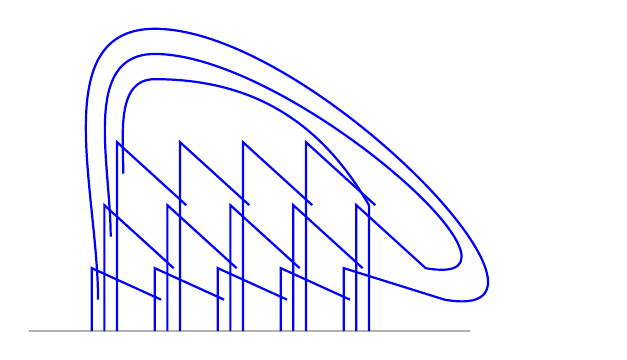
\begin{tikzpicture}[thick, scale=.8]
				\draw[Black!30] (0,0) -- (7,0);
				\foreach \i in {1,...,4}{
					\pgfmathtruncatemacro{\j}{\i+1}
					\draw[Blue] (\i,0) to (\i,1) to (\j.1,.5);
					\draw[Blue] (\i.2,0) to (\i.2,2) to (\j.3, 1);
					\draw[Blue] (\i.4,0) to (\i.4,3) to (\j.5, 2);
				}
				\draw[Blue] (5,0) to (5,1) to (6.6,.5) to[out=-10, in=0] (2,4.8) to[out=180, in=90] (1.1,.5);
				\draw[Blue] (5.2,0) to (5.2,2) to (6.3, 1) to[out=-10, in=0] (2,4.4) to[out=180, in=90] (1.3,1.5);
				\draw[Blue] (5.4,0) to (5.4,2) to[out=120, in=0] (2,4) to[out=180, in=90] (1.5,2.5);
			\end{tikzpicture}
		\end{subfigure}
		\caption{Graph on the left and on the right its representation.}
		\label{grid}
	\end{figure}
\end{proof}

\begin{thm}
	$\cn(\text{Planar}) = 3$.
\end{thm}

\begin{proof}
	For the lower bound we can use the proposition \ref{girth-cop} and draw a planar graph which has girth $\gamma = 5$, one such graph is a dodecahedron, see Fig. \ref{dodecahedron}.
	
	\begin{figure}[!ht]\centering
		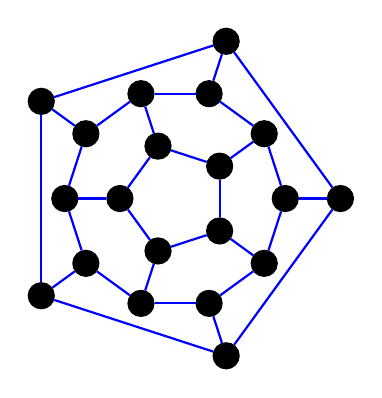
\begin{tikzpicture}[scale=.7]
			\foreach \i in {1,...,5} {
				\node[draw, circle, fill] (O-\i) at ({360/5 * (\i-1)}:3) {};
		    	}
			\foreach \i in {1,...,4} {
				\pgfmathtruncatemacro{\j}{\i+1}
				\draw[thick, Blue] (O-\i) -- (O-\j);
			}
			\draw[thick, Blue] (O-5) -- (O-1);
		       	\foreach \i in {1,...,10} {
		    		\node[draw,circle, fill] (M-\i) at ({360/10 * (\i-1)}:2) {};
		    	}
		    	\foreach \i in {1,...,9} {
				\pgfmathtruncatemacro{\j}{\i+1}
				\draw[thick, Blue] (M-\i) -- (M-\j);
			}
			\draw[thick, Blue] (M-10) -- (M-1);
		    	\foreach \i in {2,4,6,8,10} {
		    		\pgfmathtruncatemacro{\j}{\i / 2}
				\node[draw, circle, fill] (I-\j) at ({360/10 * (\i - 1)}:1) {};
		    	}
		    	\foreach \i in {1,...,4} {
				\pgfmathtruncatemacro{\j}{\i+1}
				\draw[thick, Blue] (I-\i) -- (I-\j);
			}
			\draw[thick, Blue] (I-5) -- (I-1);
			\foreach \i in {1,...,5} {
				\pgfmathtruncatemacro{\j}{2*\i}
				\pgfmathtruncatemacro{\k}{2*\i-1}
				\draw[thick, Blue] (I-\i) -- (M-\j);
				\draw[thick, Blue] (O-\i) -- (M-\k);
			}
		\end{tikzpicture}
		\caption{Dodecahedron as a planar graph.}
		\label{dodecahedron}
	\end{figure}
	
	Now for the upper bound we will show a strategy for 3 cops on connected planar graph $G$. Firstly one lemma.
	
	\begin{lemma}[cop guards path $P$]
		Let $G$ be a graph, let $P$ be a shortest path from $x$ to $y$ in $G$, $x,y \in V(G)$. Then 1 cop after finitely many moves can take position on $P$ and play a strategy that catches the robber if the robber takes any vertexof $P$.
	\end{lemma}
	
	\begin{proof}
		For simplicity denote $d(u,v)$ as the distance from $u \to v$, $c$ for cop and $r$ for robber. Strategy: If there is a vertex $w \in P$ s.t. $d(w,c) > d(w,r)$ on cops turn, then $c$ moves towards $w$, otherwise $c$ stays in place.
		
		If there is such $w$, then for $w' \in P$ on the other side of $c$ than $w$, we have $d(r,w') > d(w', c)$. Eventually, the game reaches a situation, where after every cop move $\forall w \in P : d(c,w) \leq d(r,w)$.
	\end{proof}
	
	The overview of the whole strategy is to constrain the robber by two paths and use the third cop to shrinken the graph even more. We will restrict the robber to smaller and smaller subgraphs $G = G_1 \supsetneq G_2 \supsetneq G_3 \supsetneq \dots \supsetneq \emptyset$ s.t. for $G_i$:
	
	\begin{enumerate}[I)]
		\item There are two paths $P,Q$ each guarded by 1 cop, $G_i$ is the connected component of $G \setminus (P \cup Q)$ containing the robber. $P,Q$ share the same endpoints $x_i, y_i$ and $P$ is the shortest $x_i \to y_i$ path in $G_i \cup P \cup Q$ and $Q$ is the shortest $x_i \to y_i$ path in $G_i \cup Q$. Where $G_i \cup P \cup Q$ is the same as $G_i \cup G[P] \cup G[Q]$. \label{typeI-planar-cop}
		\item There is a vertex $x$ s.t. $G_i$ is a component of $G-x$ containing the robber, $x$ is occupied by a cop. \label{typeII-planar-cop}
	\end{enumerate}
	
	Now for the strategy itself. Cops will take any vertex $x$ and robber takes any vertex $y \neq x$, let $G_2$ be the component of $G - x$ containing $y$, therefore we get type II. Now consider subcases of the starting type.
	
	\begin{itemize}[]
		\item Type \label{typeII-planar-cop}: consider few subcases.
		
		\begin{itemize}
			\item $x$ has only one neighbour $z$ in $G_i$, so put a cop there, and let $G_{i+1}$ be the component of $G_i - z$ containing the robber. Therefore we obtain again type II.
			\item $x$ has more neighbours, choose $z \neq y$ neighbour of $x_i$ in $G_i$, $P :=$ shortest $xz$-path in $G_i$. Guard $P$ with a cop and let $G_{i+1}$ be the component of $G_i \setminus P$, so we obtain type I.
		\end{itemize}
		
		\item Type I: again some subcases.
		
		\begin{itemize}
			\item If $G_i$ is adjacent to one vertex of $P \cup Q$ then we have type II. So see above case.
			\item Otherwise there is a path $R$ from $x$ to $y$ in $P \cup Q \cup G_i$, containing a vertex from $G_i$. Let $R$ be shortest such path, put cop to guard it. Afterwards either $P$ or $Q$ is no longer needed to constraint the robber so we will have free cop and smaller graph. This can be seen by dividing the face $G_i$ by the path $R$, after the cops guard all three paths then the orbber is left out in one face which is constrained by $R$ and one of $P$ or $Q$. Also we won't need to guard whole $R$ and the second path, since the face may be way smaller, only the common endpoints.
		\end{itemize}
	\end{itemize}
\end{proof}